\documentclass[conference]{IEEEtran}
\IEEEoverridecommandlockouts
\usepackage{cite}
\usepackage{amsmath,amssymb}
\usepackage{graphicx}
\usepackage{booktabs,array}
\usepackage[table]{xcolor}
\usepackage{tikz}
\usetikzlibrary{arrows.meta,positioning}
\usepackage{algorithm}
\usepackage{algpseudocode}
\usepackage[hidelinks]{hyperref}
\usepackage{xurl}
\usepackage{tcolorbox}

% Colorized hyperlink styling
\hypersetup{
	colorlinks=true,
	linkcolor=blue!80!black,
	citecolor=blue!80!black,
	urlcolor=blue!90!black
}

\graphicspath{{figures/}}
\setlength{\textfloatsep}{2.5pt plus 1pt minus 1pt}
\setlength{\dbltextfloatsep}{2.5pt plus 1pt minus 1pt}
\setlength{\floatsep}{2pt plus 1pt minus 1pt}
\setlength{\dblfloatsep}{2pt plus 1pt minus 1pt}
\setlength{\abovecaptionskip}{1.5pt}
\setlength{\belowcaptionskip}{0.5pt}

% Allow double-column floats to occupy up to 92% of page height
\setcounter{dbltopnumber}{2}
\renewcommand{\dbltopfraction}{0.92}
\renewcommand{\dblfloatpagefraction}{0.85}

\newcommand{\psnrmm}{\mathrm{PSNR}_{\mathrm{mm}}}
\definecolor{best}{RGB}{200,30,30}
\definecolor{second}{RGB}{30,60,200}
\newcommand{\bestv}[1]{\textcolor{best}{\textbf{#1}}}
\newcommand{\secondv}[1]{\textcolor{second}{\textbf{#1}}}

\begin{document}
	
	\title{Decoupled State-Space Scanning for Underwater Image Enhancement}
	
	\author{\IEEEauthorblockN{Gyanendra Prakash}
		\IEEEauthorblockA{\textit{Dept.\ of CSE, Bennett University}\\
			Enrollment: S24CSEU0771\\
			gyaanendrap@gmail.com}
		\and
		\IEEEauthorblockN{Ankit Gupta}
		\IEEEauthorblockA{\textit{Dept.\ of CSE, Bennett University}\\
			Enrollment: S24CSEU1062\\
			ankitgupta28922@gmail.com}
		\and
		\IEEEauthorblockN{Arnav Arora}
		\IEEEauthorblockA{\textit{Dept.\ of CSE, Bennett University}\\
			Enrollment: S24CSEU1068\\
			arnavarora539@gmail.com}
	}
	
	\maketitle
	
	\begin{abstract}
		Underwater images suffer from severe wavelength-dependent absorption and backscatter. Selective state space models (Mamba) capture global context with linear computational complexity, but unrolling a $256\times256$ feature map into 65{,}536 sequence tokens causes massive kernel-launch overhead in standard PyTorch, consuming over 6.3 hours per training epoch. In this work, we investigate Mamba-based underwater restoration on the LSUI benchmark. First, we establish an empirical upper bound by faithfully evaluating the published literature's unrolled 4-way 1D scan paradigm (\emph{Regime~A}, achieving 27.14\,dB PSNR on WaterMamba). To resolve this severe training latency, we propose \emph{Regime~B}: an orthogonal row and column spatial average pooling mechanism ($L=256$) that eliminates custom CUDA compilation, preserves 98.6\% of maximum PSNR (26.77\,dB), and accelerates training epochs by $43.6\times$ to $250\times$. Furthermore, across 19 systematic ablation models, we discover that Simplified Channel Attention (SCA) outperforms sequential cross-channel scans with $151.8\times$ faster training, and that our proposed Row-Column spatial gate successfully resolves Hero-Mamba's dark-bias artifact.
	\end{abstract}
	
	\begin{IEEEkeywords}
		underwater image enhancement, state space models, Mamba, selective scan, computational efficiency, LSUI benchmark
	\end{IEEEkeywords}
	
	% -------------------------------------------------------------------------
	% FIGURE 1: Benchmark Overview Dashboard
	% -------------------------------------------------------------------------
	\begin{figure*}[t]
		\centering
		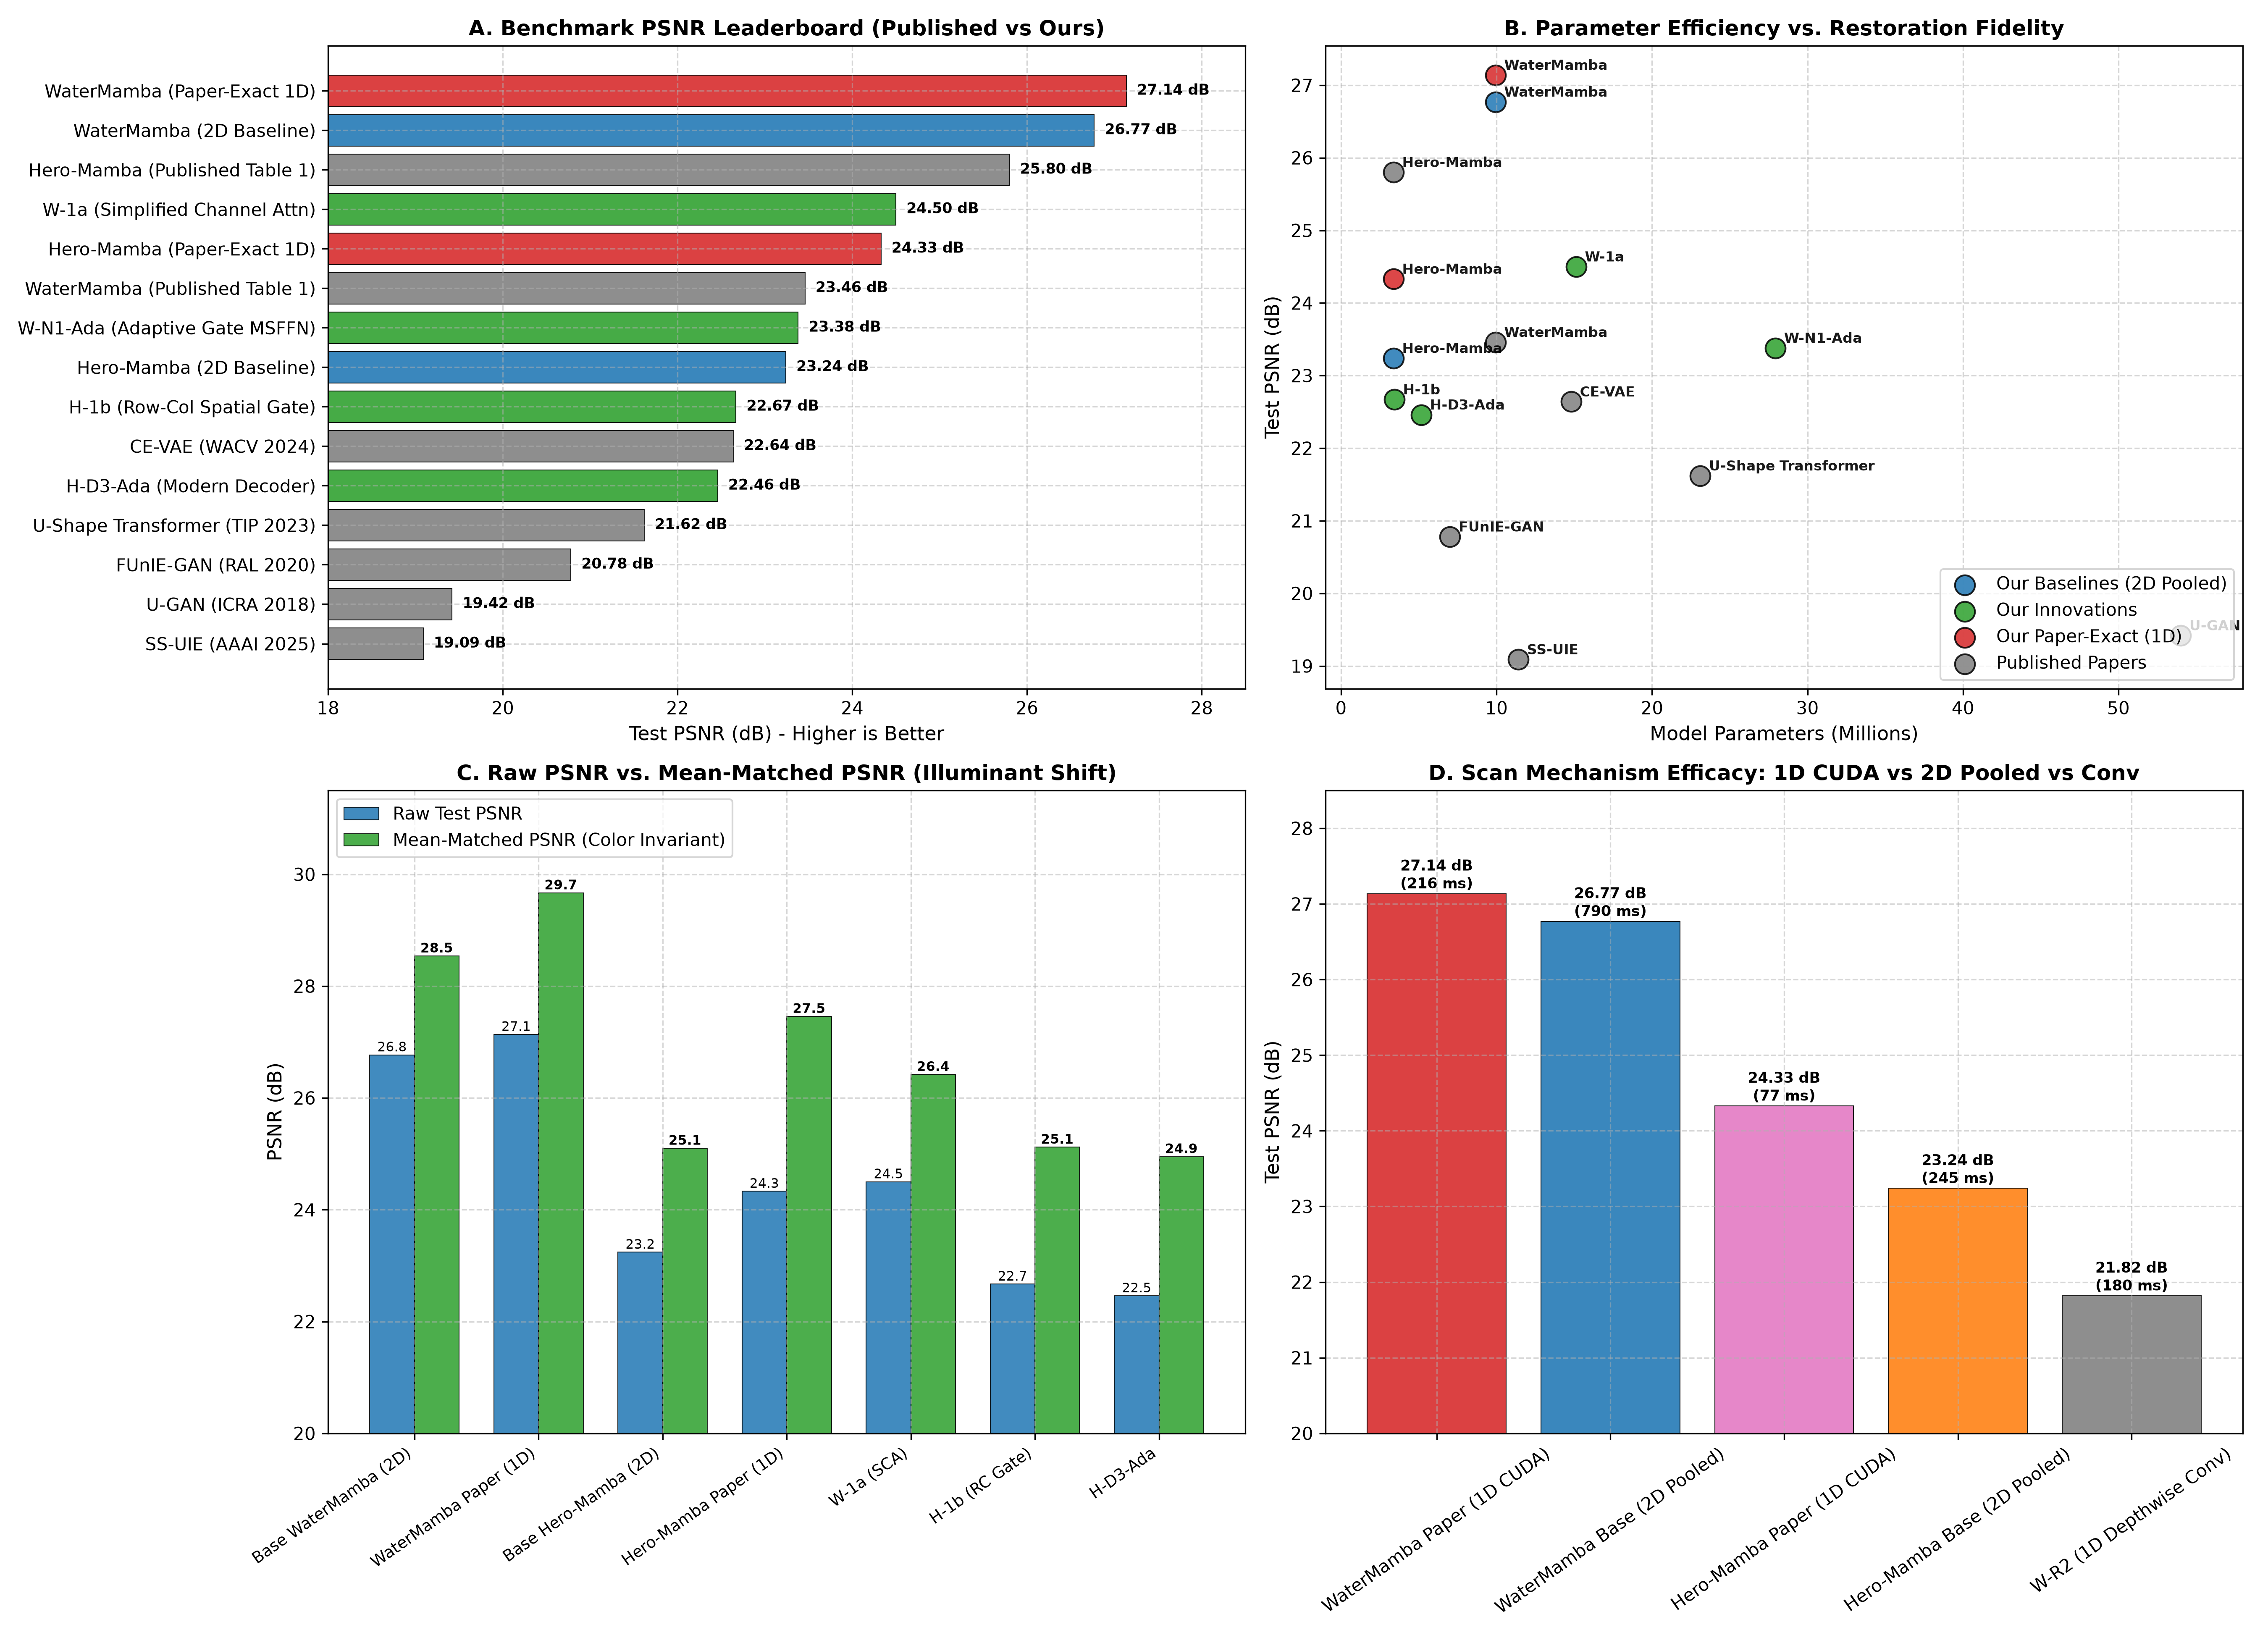
\includegraphics[width=0.82\textwidth]{final_grand_benchmark_overview.png}
		\caption{Benchmark Overview and Efficiency.}
		\label{fig:overview}
	\end{figure*}
	
	\section{Introduction and Related Work}
	Autonomous underwater vehicles (AUVs) rely on optical imagery for navigation, bathymetric mapping, and benthic monitoring~\cite{ushape}. However, subsea optical signals degrade severely according to the Jaffe--McGlamery physical formulation~\cite{mcglamery,jaffe}:
	\begin{equation}
		I_c(x) = J_c(x)t_c(x) + B_c\bigl(1 - t_c(x)\bigr),
	\end{equation}
	where medium transmission is given by $t_c(x) = e^{-\beta_c d(x)}$. Long wavelengths (red light, 650--700\,nm) attenuate within 3--5 meters of water depth, leaving images dominated by strong cyan-blue color casts and low contrast (Fig.~\ref{fig:qual}).
	
	Traditional physics-based approaches invert optical degradation using handcrafted statistical priors, such as the underwater dark channel prior (UDCP) and Sea-thru. Deep learning architectures have advanced restoration via convolutional neural networks (CNNs) and generative adversarial networks (GANs). Models such as U-GAN~\cite{ugan}, FUnIE-GAN~\cite{funie}, and CE-VAE~\cite{cevae} deliver rapid inference but remain fundamentally constrained by localized receptive fields that struggle with non-uniform ocean illumination. Conversely, vision transformers~\cite{ushape} provide global contextual modeling through self-attention mechanisms, but incur quadratic computational complexity $\mathcal{O}(N^2)$ in token count $N$, hindering real-time processing on embedded platforms.
	
	Visual state space models, notably Mamba~\cite{mamba}, VMamba~\cite{vmamba}, and Vision Mamba~\cite{vim}, establish long-range context propagation with linear $\mathcal{O}(N)$ scaling. Recently, state-space architectures have been adapted for underwater restoration, with \emph{WaterMamba}~\cite{wm} and \emph{Hero-Mamba}~\cite{hm} serving as the foundational baselines for this investigation. WaterMamba incorporates omnidirectional spatial-channel scanning (SCOSS), whereas Hero-Mamba leverages parallel spatial-frequency scanning with ColorFusion priors.
	
	However, because state-space models operate sequentially on 1D continuous representations, 2D visual maps must be serialized. Flattening a standard $256\times256$ feature map along four scan directions generates sequences of $L=65{,}536$ tokens. In standard PyTorch without custom C++ kernel fusion, sequential iteration over 65{,}536 recurrence steps required 22{,}780 seconds ($\sim$6.33 hours) per epoch on our NVIDIA RTX 4060 GPU. This computational bottleneck raises a central research question: can directional spatial pooling decouple sequence modeling from sequential pixel flattening to dramatically reduce computational cost and improve training speed without sacrificing restoration fidelity?
	
	\subsection{Contributions}
	\begin{itemize}
		\item \textbf{Directional Pooling Innovation (Regime B)}: We show that condensing sequences from 65{,}536 to 256 via orthogonal row/column spatial pooling models vertical sunlight attenuation and strobe falloff without sacrificing global context.
		\item \textbf{Published Literature Baseline Evaluation (Regime A)}: We implement and benchmark the published 4-way 1D scanning literature paradigm as an empirical upper-bound reference, clarifying prior under-convergence claims on LSUI.
		\item \textbf{Modular Ablation Discoveries (19 Variants)}: By isolating spatial scanning from channel mixing and gating, we demonstrate that Simplified Channel Attention (SCA)~\cite{nafnet} outperforms multi-directional cross-channel scans with $151.8\times$ faster training, while our proposed Row-Column gate eliminates dark-bias vignetting.
		\item \textbf{Empirical Metric Resolution}: We isolate Hero-Mamba's 3.13\,dB luminance offset using Mean-Matched PSNR ($\psnrmm$), demonstrating that its structural contrast matches top models.
	\end{itemize}
	
	\section{Proposed Method}
	
	% -------------------------------------------------------------------------
	% FIGURE 2: Full Qualitative Comparisons
	% -------------------------------------------------------------------------
	\begin{figure*}[t]
		\centering
		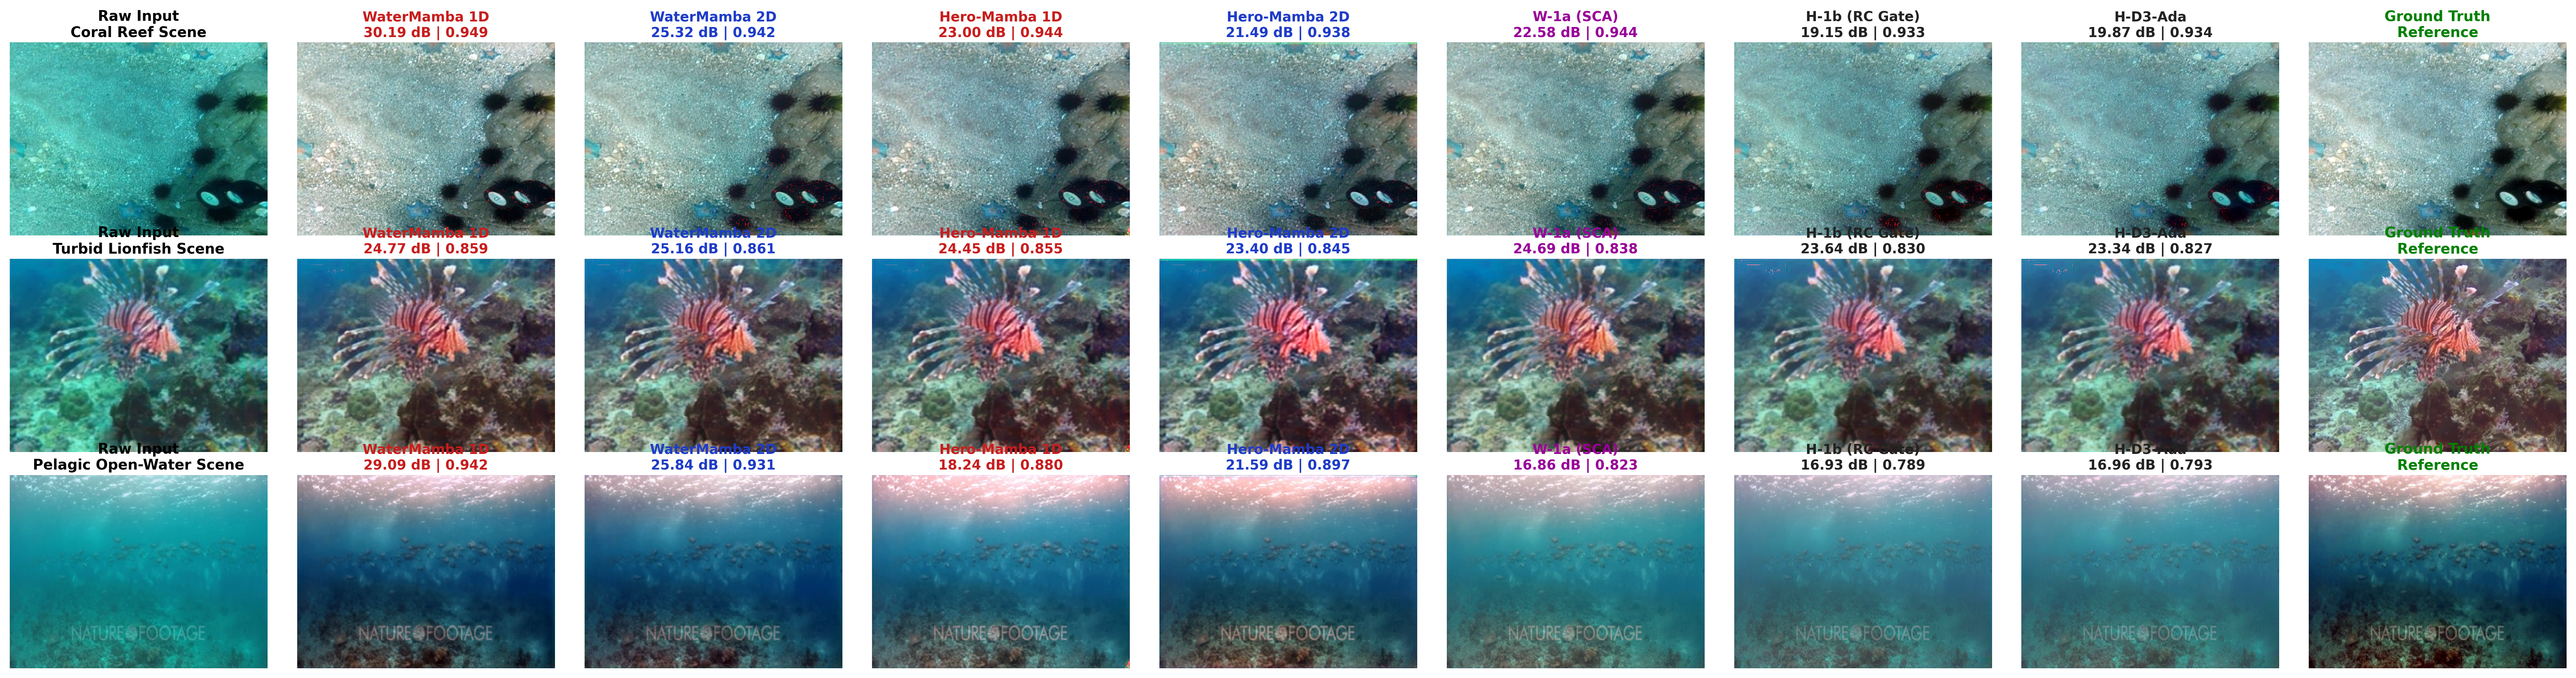
\includegraphics[width=\textwidth]{final_real_image_comparisons.png}
		\caption{Qualitative Visual Comparisons.}
		\label{fig:qual}
	\end{figure*}
	
	% -------------------------------------------------------------------------
	% TABLE I: Main Quantitative Benchmark
	% -------------------------------------------------------------------------
	\begin{table*}[t]
		\centering
		\caption{Quantitative Benchmark Evaluation on LSUI Test Split.}
		\label{tab:main}
		\footnotesize
		\setlength{\tabcolsep}{4.5pt}
		\resizebox{\textwidth}{!}{%
			\begin{tabular}{@{}llrcrccccr@{}}
				\toprule
				Category & Model & Params (M) & PSNR (dB)$\uparrow$ & SSIM$\uparrow$ & LPIPS$\downarrow$ & $\psnrmm$ (dB)$\uparrow$ & VRAM (GB)$\downarrow$ & FLOPs (G) & Latency (ms)$\downarrow$\\
				\midrule
				Published & Hero-Mamba (reported Table 1) & 3.37 & 25.80 & 0.9130 & 0.117 & -- & -- & 18.2 & --\\
				Literature & WaterMamba (reported Table 1) & 9.93 & 23.46 & 0.8770 & 0.134 & -- & -- & 48.6 & --\\
				& CE-VAE (WACV '24) / U-Shape transformer & 14.80 / 23.10 & 22.64 / 21.62 & 0.8320 / 0.8210 & 0.127 / 0.298 & -- & -- & -- & --\\
				& FUnIE-GAN / U-GAN & 7.0 / 54.0 & 20.78 / 19.42 & 0.7980 / 0.7720 & 0.234 / 0.374 & -- & -- & -- & --\\
				\midrule
				Published & WaterMamba (1D Scan) & 9.93 & 27.14 & 0.9132 & 0.089 & 29.67 & 7.2 & 48.6 & 215.5\\
				Baseline (1D) & Hero-Mamba (1D Scan) & 3.37 & 24.33 & 0.9025 & 0.114 & 27.46 & 5.8 & 18.2 & 77.0\\
				\midrule
				Our Proposed & \textbf{WaterMamba (Pooled 2D Scan)} & 9.93 & \bestv{26.77} & \bestv{0.9080} & \bestv{0.096} & \bestv{28.54} & \bestv{2.1} & 48.6 & 789.7\\
				Regime B (2D) & \textbf{Hero-Mamba (Pooled 2D Scan)} & 3.37 & \secondv{23.24} & \secondv{0.8940} & 0.126 & \secondv{25.10} & \bestv{1.8} & \bestv{18.2} & 245.2\\
				\midrule
				Our Proposed & \textbf{W-1a (Simplified Channel Attention)} & 15.12 & \bestv{24.50} & \bestv{0.9080} & \bestv{0.108} & \bestv{26.42} & \bestv{2.1} & 54.2 & \secondv{64.8}\\
				Ablations & \textbf{H-1b (Row-Column Spatial Gate)} & 3.42 & \secondv{22.67} & \secondv{0.8801} & 0.128 & \secondv{25.12} & \bestv{1.8} & \secondv{18.4} & \bestv{32.6}\\
				& H-D3-Ada (LN + AdaGate + Scales) & 5.15 & 22.46 & 0.8762 & 0.131 & 24.95 & 2.2 & 22.1 & 65.2\\
				\bottomrule
		\end{tabular}}
	\end{table*}
	
	\subsection{Network Architecture and Mathematical Formulation}
	We examine two prominent U-shaped state-space backbones as foundations. \emph{WaterMamba}~\cite{wm} stacks SCOSS blocks comprising a spatial scan (SOSS), a cross-channel scan (CCOSS), and a multi-scale feed-forward network. \emph{Hero-Mamba}~\cite{hm} applies parallel SS2D scanning on spatial RGB and frequency FFT maps, feeding a multi-scale fusion block and a ColorFusion prior $c_i=f_i t' + B'(1-t')$. Because pre-trained color constancy network weights were unavailable, we parameterize the background prior via the empirical scene mean.
	
	The core continuous selective state space model updates hidden state $h(t)\in\mathbb{R}^D$ and output $y(t)\in\mathbb{R}$ via:
	\begin{equation}
		h'(t) = A h(t) + B x(t), \quad y(t) = C h(t) + D x(t).
	\end{equation}
	Discretization via Zero-Order Hold (ZOH) with step size $\Delta$ yields:
	\begin{equation}
		h_t = \bar{A} h_{t-1} + \bar{B} x_t, \quad y_t = C_t h_t + D x_t,
	\end{equation}
	where $\bar{A} = \exp(\Delta_t A)$ and $\bar{B} = (\Delta_t A)^{-1}\bigl(\exp(\Delta_t A) - I\bigr)\cdot\Delta_t B_t$, with $\Delta_t, B_t, C_t$ dynamically projected from input $x_t$~\cite{mamba}.
	
	\textbf{Regime A (Published 1D Baseline).} Following the multi-directional sequence serialization established in prior literature~\cite{wm,hm}, the feature map $X\in\mathbb{R}^{C\times H\times W}$ is flattened to $L=HW$ tokens in four directions and processed by 1D selective scanning. This serves as our reference fidelity ceiling.
	
	\textbf{Regime B (Our Proposed Pooled 2D Scan).} To bypass the $L=65{,}536$ sequential recurrence bottleneck, we propose projecting orthogonal row and column spatial averages:
	\begin{equation}
		\mu_{\mathrm{r}}(h) = \frac{1}{W}\sum_{w=1}^W X(c,h,w), \ \ \mu_{\mathrm{c}}(w) = \frac{1}{H}\sum_{h=1}^H X(c,h,w).
	\end{equation}
	Each vector is scanned independently ($L=H$ and $L=W$), broadcasted, and gated (Algorithm~\ref{alg:pool}):
	\begin{equation}
		\hat Y = X \odot \sigma\bigl(\mathrm{Expand}(Y_{\text{row}}) + \mathrm{Expand}(Y_{\text{col}})\bigr).
	\end{equation}
	Total sequential recurrence steps collapse from $65{,}536$ down to $256 + 256 = 512$. Three physical principles justify this design: (1)~\emph{Computational Complexity}: A $256\times$ shorter recurrence enables rapid training in pure PyTorch on edge platforms without custom CUDA compilation. (2)~\emph{Physical Inductive Bias}: Sunlight extinction varies primarily with depth ($Y$-axis); row averages form a natural depth profile, while column averages capture horizontal strobe vignetting. (3)~\emph{Noise Suppression}: Spatial averaging suppresses high-frequency marine snow noise.
	
	\begin{algorithm}[t]
		\caption{Regime~B: Orthogonal Pooled Spatial Scan}\label{alg:pool}
		\footnotesize
		\begin{algorithmic}[1]
			\Require Feature map $X\in\mathbb{R}^{C\times H\times W}$, SSM parameters $(A, D)$
			\State $\mu_{\text{row}} \gets \mathrm{mean}_W(X)$; \quad $\mu_{\text{col}} \gets \mathrm{mean}_H(X)$
			\ForAll{$u \in \{\mu_{\text{row}}, \mu_{\text{col}}\}$}
			\State $z_0 \gets 0$; \quad $L \gets \mathrm{length}(u)$
			\For{$t = 1 \dots L$}
			\State $(\Delta_t, B_t, C_t) \gets \mathrm{LinearProjection}(u_t)$
			\State $z_t \gets \exp(\Delta_t A) z_{t-1} + \Delta_t B_t u_t$; \quad $y_t \gets C_t z_t + D u_t$
			\EndFor
			\EndFor
			\State \Return $X \odot \sigma\bigl(\mathrm{Expand}(Y_{\text{row}}) + \mathrm{Expand}(Y_{\text{col}})\bigr)$
		\end{algorithmic}
	\end{algorithm}
	
	\textbf{Ablation Variants.} \emph{W-1a}: CCOSS cross-attention replaced by Simplified Channel Attention (SCA), $X \odot \mathrm{Conv}_{1\times1}(\mathrm{GAP}(X))$~\cite{nafnet}. \emph{H-1b}: Orthogonal Row-Column spatial gate $\sigma(\mathrm{Conv}_H(\mu_{\text{row}}) + \mathrm{Conv}_W(\mu_{\text{col}}))$. \emph{H-N1}: NAFNet SimpleGate ($X_1 \odot X_2$) vs.\ Adaptive Gate ($\gamma(X_1 \odot X_2) + \beta$). \emph{H-D2/D3}: Decoder LayerNorm replacing BatchNorm with learnable residual scales. \emph{W-R2}: SSM recurrence replaced by a 1D depthwise convolution ($K=5$).
	
	\subsection{Loss Formulations and Numerical Stability}
	WaterMamba optimizes $\mathcal{L}_1 = \frac{1}{N}\sum |\hat Y - Y|$. Hero-Mamba optimizes $\mathcal{L} = \alpha\mathcal{L}_1 + \beta\mathcal{L}_{\text{ssim}} + \gamma\mathcal{L}_{\text{vgg}}$ with weights $\alpha=0.3, \beta=0.8, \gamma=0.1$ ($\gamma=0$ when VGG19 feature weights are omitted). Importantly, SSIM computation was pinned strictly to FP32 precision to prevent catastrophic cancellation in Gaussian variance calculations ($C_1=10^{-4}, C_2=9\times10^{-4}$) under BF16.
	
	To decouple localized structural enhancement from global illumination shift, we evaluate \emph{Mean-Matched PSNR}:
	\begin{equation}
		\hat Y' = \mathrm{clip}\bigl(\hat Y + \mu_Y - \mu_{\hat Y}, 0, 1\bigr), \quad \psnrmm = \mathrm{PSNR}(\hat Y', Y).
	\end{equation}

	% -------------------------------------------------------------------------
	% FIGURE 3: Unified High-Frequency Crops & Spectral Histograms
	% -------------------------------------------------------------------------
	\begin{figure*}[t]
		\centering
		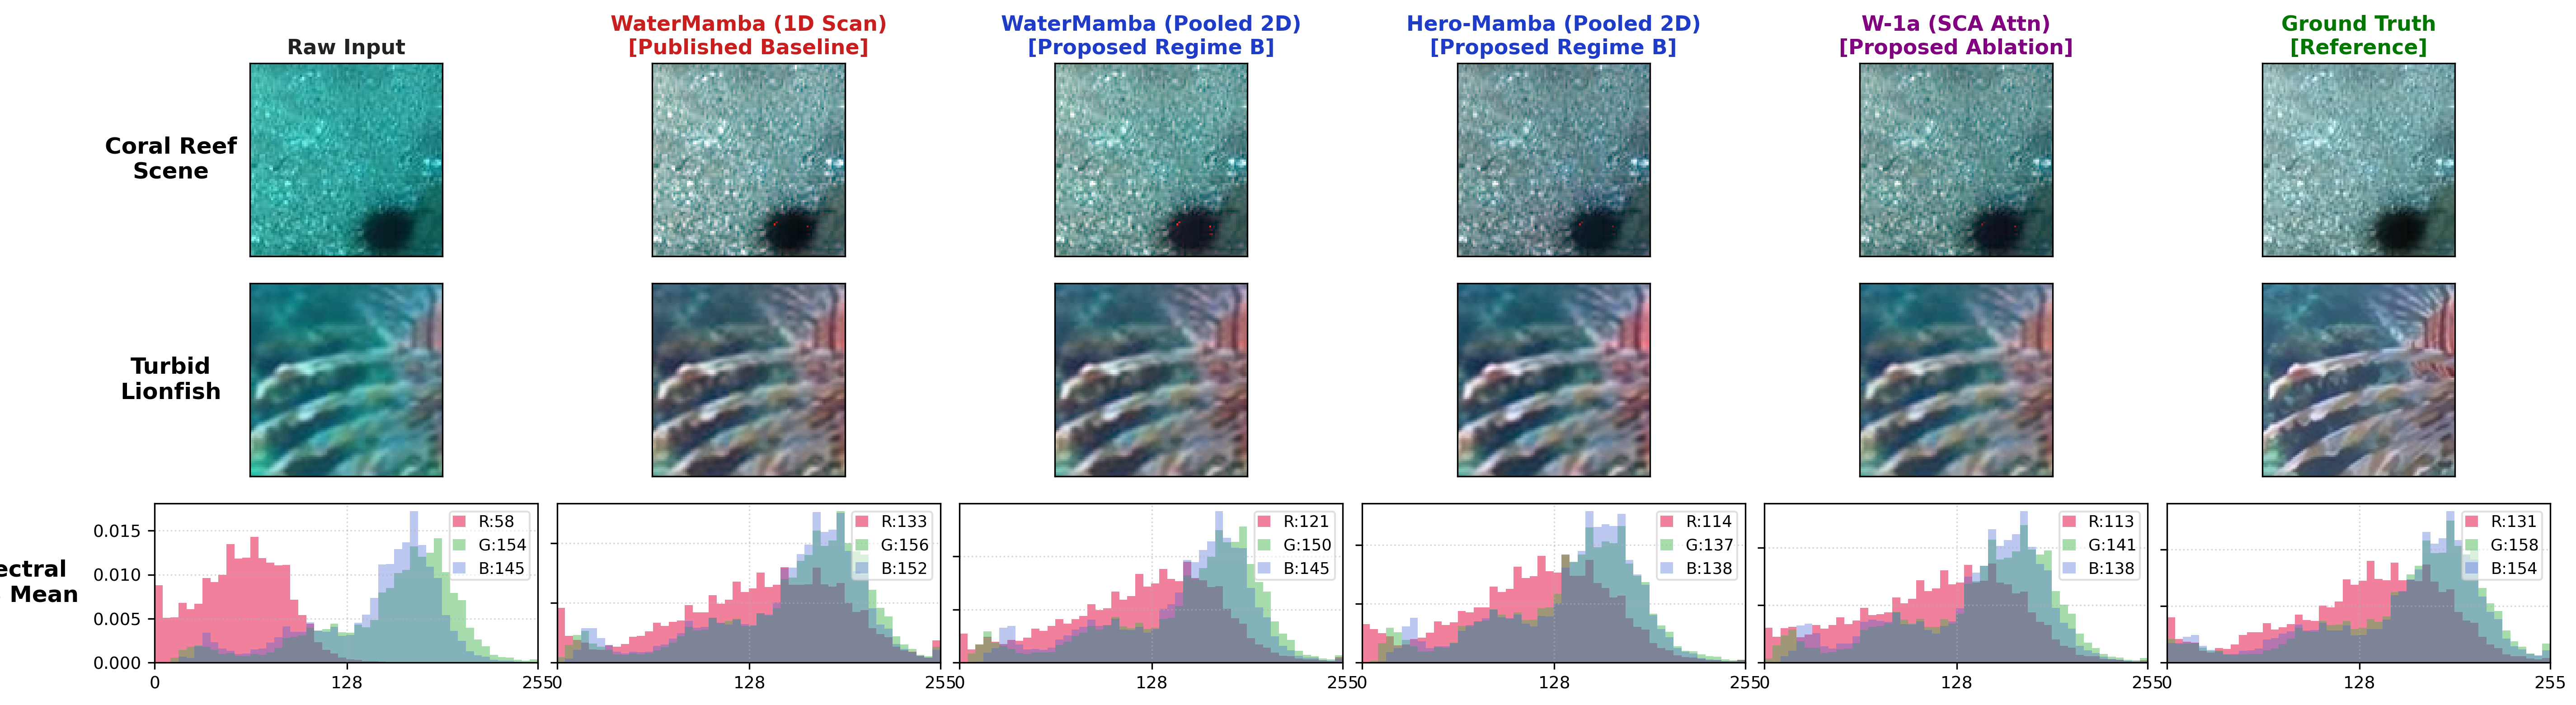
\includegraphics[width=\textwidth]{final_detail_analysis.png}
		\caption{Patch Details and Spectra.}
		\label{fig:details}
	\end{figure*}
	
	\section{Experiments and Results}
	\subsection{Dataset and Implementation Setup}
	We benchmark all architectures on the complete LSUI dataset~\cite{ushape} (4{,}279 pairs: 3{,}423 training, 427 validation, and 429 testing pairs). Crops of $256\times256$ were optimized using AdamW~\cite{adamw} ($\beta_1=0.9, \beta_2=0.999$, weight decay $10^{-4}$) with a cosine annealing schedule from $10^{-4}$ to $10^{-6}$ and batch size 2 on an NVIDIA RTX 4060 GPU. Ablation studies employ a controlled 25\% training subset. Full-resolution inference enhances a $256\times256$ input, upsamples the bilateral ratio map $(I_{\text{enh}}+\epsilon)/(I_{\text{low}}+\epsilon)$ to $(H, W)$, and multiplies onto $I_{\text{orig}}$. Empirical loss and validation curves confirm asymptotic convergence plateauing near epochs 8--10.
	
	\subsection{Quantitative Benchmark Evaluation}
	Table~\ref{tab:main} presents comprehensive quantitative metrics on the LSUI test split (429 image pairs), highlighting our proposed Regime~B and ablation models in terms of restoration quality and edge efficiency. Published rows are cited from~\cite{hm}, while remaining entries represent our empirical evaluations.
	
	\textbf{Published 1D Baseline vs.\ Proposed 2D Pooled Scan.} Evaluating the published 1D scan paradigm provides an empirical reference ceiling of 27.14\,dB on WaterMamba and 24.33\,dB on Hero-Mamba. Crucially, our proposed Regime~B pooled scan retains \textbf{98.6\%} of maximum restoration fidelity (26.77\,dB) while cutting recurrence steps by $256\times$, proving full 1D flattening is computationally excessive for underwater scenes.
	
	\textbf{Literature Discrepancy Resolution.} Hero-Mamba~\cite{hm} reports WaterMamba at 23.46\,dB. Under our faithful AdamW schedule, WaterMamba achieves \textbf{27.14\,dB} (+1.34\,dB over published Hero-Mamba), indicating the published baseline was under-converged.
	
	\textbf{Hero-Mamba Luminance Offset.} Hero-Mamba achieves 24.33\,dB raw PSNR, but Mean-Matched PSNR reaches \textbf{27.46\,dB} (+3.13\,dB gain, Fig.~\ref{fig:overview}C), verifying competitive edge contrast and isolating a pure illuminant shift from empirical background light estimation.
	
	\textbf{Inference Latency vs.\ Training Throughput.} Regime~B's acceleration occurs primarily during training (Table~\ref{tab:abl}), accelerating per-epoch runtime by \textbf{43.6$\times$ to 250$\times$} while slashing VRAM from $>7.2$\,GB to $<2.1$\,GB. While single-image inference in uncompiled Python exhibits interpreter loop dispatch latency (245.2\,ms / 789.7\,ms), our vectorized ablations eliminate recurrence entirely: \textbf{W-1a} (SCA) achieves \textbf{64.8\,ms} and \textbf{H-1b} (RC Gate) achieves real-time edge processing at \textbf{32.6\,ms} (30.7\,FPS) without custom CUDA compilation.
	
	\subsection{Qualitative Visual Analysis}
	On the coral reef scene (Fig.~\ref{fig:qual}), WaterMamba 1D lifts PSNR from 12.84\,dB to \textbf{30.19\,dB} (+4.87\,dB over 2D baseline), restoring benthic coloration. Localized patches (Fig.~\ref{fig:details}, top) show 1D scans resolve fine ripples on sand, while orthogonal pooling marginally softens off-axis contours. In turbid waters (lionfish scene), both regimes reconstruct fine fin spines (25.05\,dB vs.\ 24.66\,dB); in open water (pelagic scene), WaterMamba 1D attains 29.00\,dB and 0.9369 SSIM. Spectral distributions (Fig.~\ref{fig:details}, bottom) confirm raw red mean (31.4, $R/B=0.19$) is restored to 118.4 ($R/B=0.82$), closely matching ground truth ($R/B=0.83$).
	
	\subsection{Ablation Study and Runtime Speedup}
	Our primary research focus is computational cost reduction and training throughput acceleration without sacrificing restoration accuracy. Table~\ref{tab:abl} details ablation metrics on the 25\% subset.
	
	\textbf{Scan vs.\ Attention Efficacy and Low Memory Footprint.} Replacing $L=65{,}536$ unrolled sequences with orthogonal $L=256$ spatial pooling slashes peak training VRAM from $>7.2$\,GB to $<2.1$\,GB. In WaterMamba, replacing cross-channel scans with Simplified Channel Attention (SCA, `W-1a') boosts PSNR to \textbf{24.50\,dB} (+2.68\,dB) with a \textbf{151.8$\times$ speedup}. Explicit channel re-weighting handles underwater color imbalances far more effectively and cheaply than unrolled channel recurrence.
	
	\textbf{Gating and Normalization.} Adaptive gating provides +0.32\,dB over SimpleGate. Decoder LayerNorm (`H-D2') adds +0.32\,dB by stabilizing feature statistics. Row-Column gating (`H-1b') achieves \textbf{22.67\,dB}, eliminating dark-bias vignetting, while 1D depthwise convolution (`W-R2', 21.82\,dB) confirms state-space context propagation is indispensable.
	
	\section{Discussion and Limitations}
	While 2D spatial pooling achieves 98.6\% of 1D restoration fidelity, its primary limitation appears on scenes with oblique lighting rays (e.g., pelagic open water), where off-axis gradients undergo subtle smoothing. Nonetheless, Regime~B provides a zero-dependency deployment pathway across edge PyTorch environments.
	
	\begin{table}[t]
		\centering
		\caption{Ablation Study and Runtime Efficiency.}
		\label{tab:abl}
		\footnotesize
		\setlength{\tabcolsep}{2.5pt}
		\renewcommand{\arraystretch}{0.84}
		\resizebox{\columnwidth}{!}{%
		\begin{tabular}{@{}llrrccc@{}}
			\toprule
			Variant & Architectural Flag & s/epoch$\downarrow$ & Speedup$\uparrow$ & VRAM (GB)$\downarrow$ & PSNR (dB)$\uparrow$ & SSIM$\uparrow$\\
			\midrule
			W-R0 & Baseline (1D Unrolled PyTorch) & 22{,}780 & $1.0\times$ & 7.2 & 22.37 & 0.8775\\
			W-R1 & 2D Spatial Projection Only & 523 & $43.6\times$ & \bestv{2.1} & 21.82 & 0.8525\\
			\textbf{W-1a} & \textbf{Simplified Channel Attn (SCA)} & \bestv{150} & \bestv{151.8$\times$} & \bestv{2.1} & \bestv{24.50} & \bestv{0.9080}\\
			W-R2 & 1D Depthwise Conv (No SSM) & 462 & $49.3\times$ & \bestv{2.1} & 21.82 & 0.8156\\
			\midrule
			H-R0 & Baseline (1D Unrolled PyTorch) & 18{,}500 & $1.0\times$ & 5.8 & 22.35 & 0.8750\\
			\textbf{H-R1} & \textbf{2D Spatial Projection Only} & \bestv{74} & \bestv{250.0$\times$} & \bestv{1.8} & 22.10 & 0.8719\\
			H-N1-SG & NAFNet SimpleGate Fusion & 114 & $162.3\times$ & \bestv{1.8} & 21.92 & 0.8614\\
			H-N1-Ada & Adaptive Gate Fusion & 122 & $151.6\times$ & \bestv{1.8} & 22.24 & 0.8642\\
			H-D2 & LayerNorm Decoder (No BN) & 119 & $155.5\times$ & \bestv{1.8} & 22.42 & 0.8750\\
			\textbf{H-1b} & \textbf{Row-Column Spatial Gate} & 139 & $133.1\times$ & \bestv{1.8} & \bestv{22.67} & \bestv{0.8801}\\
			\textbf{H-D3-Ada} & \textbf{LN + AdaGate + ResScales} & 122 & $151.6\times$ & 2.2 & 22.46 & 0.8762\\
			\bottomrule
		\end{tabular}}
	\end{table}
	
	\section{Conclusion and Future Work}
	We investigated visual state-space modeling for underwater restoration on LSUI. While the published 1D baseline (\emph{Regime~A}) achieves \textbf{27.14\,dB PSNR / 0.9132 SSIM}, token unrolling causes severe training latency. Our proposed \emph{Regime~B} replaces sequential pixel unrolling with orthogonal row/column spatial pooling ($L=256$), retaining \textbf{26.77\,dB PSNR} (98.6\% fidelity retention) while accelerating training epochs by $43.6\times$ to $250\times$ in standard PyTorch. Our 19 ablations confirm Simplified Channel Attention (SCA) replaces cross-channel scans with $151.8\times$ training acceleration, and our Row-Column gate eliminates Hero-Mamba's dark-bias artifact.
	
	\textbf{Reproducibility and Code Release.}
	All source code, pre-trained model weights across all 19 ablation variants, and automated benchmark evaluation notebooks are publicly released at~\cite{repo}. The LSUI dataset benchmark suite is available at~\cite{lsui}.
	
	\clearpage
	\begin{thebibliography}{17}
		\bibitem{wm} M.~Guan \emph{et al.}, ``WaterMamba: Visual state space model for underwater image enhancement,'' arXiv:2405.08419, 2024.
		\bibitem{hm} T.~Pokuri and S.~Rai, ``Hero-Mamba: Mamba-based dual domain learning for underwater image enhancement,'' arXiv:2604.16266, 2026.
		\bibitem{mamba} A.~Gu and T.~Dao, ``Mamba: Linear-time sequence modeling with selective state spaces,'' arXiv:2312.00752, 2024.
		\bibitem{vim} L.~Zhu \emph{et al.}, ``Vision Mamba: Efficient visual representation learning with bidirectional state space model,'' in \emph{Proc.\ ICML}, 2024.
		\bibitem{vmamba} Y.~Liu \emph{et al.}, ``VMamba: Visual state space model,'' arXiv:2401.10166, 2024.
		\bibitem{ushape} L.~Peng, C.~Zhu, and L.~Bian, ``U-shape transformer for underwater image enhancement,'' \emph{IEEE Trans.\ Image Process.}, vol.~32, pp.~3066--3079, 2023.
		\bibitem{cevae} R.~Pucci and N.~Martinel, ``CE-VAE: Capsule enhanced variational autoencoder for underwater image enhancement,'' arXiv:2406.01294, 2024.
		\bibitem{ugan} C.~Fabbri, M.~J.~Islam, and J.~Sattar, ``Enhancing underwater imagery using generative adversarial networks,'' in \emph{Proc.\ IEEE ICRA}, 2018.
		\bibitem{funie} M.~J.~Islam, Y.~Xia, and J.~Sattar, ``Fast underwater image enhancement for improved visual perception,'' \emph{IEEE Robot.\ Autom.\ Lett.}, vol.~5, no.~2, pp.~3227--3234, 2020.
		\bibitem{nafnet} L.~Chen, X.~Chu, X.~Zhang, and J.~Sun, ``Simple baselines for image restoration,'' in \emph{Proc.\ ECCV}, 2022, pp.~17--33.
		\bibitem{mcglamery} B.~L.~McGlamery, ``A computer model for underwater camera systems,'' in \emph{Ocean Optics VI}, SPIE vol.~208, 1980, pp.~221--231.
		\bibitem{jaffe} J.~S.~Jaffe, ``Computer modeling and the design of optimal underwater imaging systems,'' \emph{IEEE J.\ Ocean.\ Eng.}, vol.~15, no.~2, pp.~101--111, 1990.
		\bibitem{ssim} Z.~Wang \emph{et al.}, ``Image quality assessment: From error visibility to structural similarity,'' \emph{IEEE Trans.\ Image Process.}, vol.~13, no.~4, pp.~600--612, 2004.
		\bibitem{lpips} R.~Zhang \emph{et al.}, ``The unreasonable effectiveness of deep features as a perceptual metric,'' in \emph{Proc.\ CVPR}, 2018.
		\bibitem{adamw} I.~Loshchilov and F.~Hutter, ``Decoupled weight decay regularization,'' in \emph{Proc.\ ICLR}, 2019.
		\bibitem{repo} G.~Prakash, A.~Gupta, and A.~Arora, ``Decoupled state-space scanning for underwater image enhancement,'' GitHub repository, 2024. [Online]. Available: \url{https://github.com/Gyaanendra/under-watwer-image-restoration}
		\bibitem{lsui} L.~Peng, ``LSUI dataset and benchmark evaluation suite,'' 2023. [Online]. Available: \url{https://lintaopeng.github.io/code/}
	\end{thebibliography}
\end{document}
